\section{Temporal Results and Analysis}

\subsection{Hyperparameter Optimization}
The grid of Passive-Aggressive Regressor models that perform the temporal predictions have several hyperparameters that need optimization to fit better with the application and obtain better results. Only data from static sensors of dataset A was used for optimization. The approach used was grid search across three different variables: C, epsilon and loss as explained in section \ref{chap:par} and the values experimented are listed in Table \ref{tab:hyperparams}.

\begin{table}[H]
\centering
\resizebox{\textwidth}{!}{%
\begin{tabular}{|c|c|c|}
\textbf{Hperparameter "C"} & \textbf{Hyperparameter "epsilon"} & \textbf{Hyperparameter "loss"} \\
\multicolumn{1}{|l|}{} & \multicolumn{1}{l|}{} & \multicolumn{1}{l|}{} \\
$\num{2e-7}$ & $\num{1e-3}$ & squared\_epsilon\_insensitive \\
$\num{2e-5}$ & $\num{1e-1}$ & epsilon\_insensitive \\
$\num{2e-4}$ & $\num{5e-1}$ &  \\
$\num{2e-3}$ & 1 &  \\
$\num{2e-2}$ & 2.5 &  \\
$\num{2e-1}$ & 5 &  \\
2 &  & 
\end{tabular}%
}
\caption{List of hyperparameters used in grid search method}
\label{tab:hyperparams}
\end{table}

The experiment was done independently for each static sensor in order to investigate if there were benefits of having independently adjusted hyperparameter settings for each cell or if the same configuration could be used throughout the grid. Purely from a programming perspective, the same set of hyperparameters in all cells would be a better design decision as it provides simplicity to the model and helps define hyperparameters in grid cells where not enough data is available, or data does not exist at all. As results demonstrate in Table \ref{tab:hyperresults}, there is a minimal improvement of performance when a different set of hyperparameters is applied to each square compared to having the same set of hyperparameters in the whole grid, 0.158 and 0.159 respectively.
This experiment demonstrated the best set of hyperparameters to be $C= \num{2e-5}$, $epsilon = 0.001$ and $loss = epsilon\_insensitive$.

In a real-time context, it could be useful to recompute the hyperparameters of the model from time to time to adapt to possible changes due to long term seasonal changes in the environment.

\begin{table}[h]
\centering
\resizebox{\textwidth}{!}{%
\begin{tabular}{c|c|c|c|c|c}
\textbf{Sensor Name} & Best C value & Best epsilon value & Best loss value & \textbf{Mean Absolute Error} & \multicolumn{1}{l}{\textbf{Mean Squared Error}} \\ \hline
Lauriston & $\num{2e-5}$ & 0.001 & epsilon\_insensitive & 0.125 & 0.031 \\
Melville & $\num{2e-5}$ & 0.1 & epsilon\_insensitive & 0.400 & 0.296 \\
Tennis Court & 0.2 & 0.001 & epsilon\_insensitive & 0.076 & 0.013 \\
Library & $\num{2e-5}$ & 0.001 & epsilon\_insensitive & 0.122 & 0.035 \\
Bristo Square & 2 & 0.001 & epsilon\_insensitive & 0.114 & 0.036 \\
Buccleuch Place & 2 & 0.001 & epsilon\_insensitive & 0.108 & 0.021 \\ \hline
\textbf{Average} & - & - & - & \textbf{0.158} & \textbf{0.072} \\ \hline
\textbf{\begin{tabular}[c]{@{}c@{}}Best values\\ for all sensors\end{tabular}} & \textbf{$\num{2e-5}$} & \textbf{0.001} & \textbf{epsilon\_insensitive} & \textbf{0.159} & \textbf{0.076} \\ \hline
\end{tabular}%
}
\caption{Grid search results}
\label{tab:hyperresults}
\end{table}

\subsection{Features of PAR model}
The results presented in Table \ref{tab:hyperresults} refer to a PAR model that only includes time as an input feature. However another set of features was experimented: one that included temperature, humidity and last PM2.5 value as features. The same hyperparameter optimization was executed (except attempt with $C=\num{2e-7}$). That experiment yielded a minimum MAE of $0.769$ and MSE of $1.21$, in the case $"C"= \num{2e-5}$, $"epsilon" = 0.5$ and $"loss" = epsilon\_insensitive$. Because of these results, this model was not explored further and the other model was used as the temporal model.

\subsection{Data noise reduction}

Figure \ref{fig:resamples} shows the data collected from one static sensor, resampled at different time durations. These four figures show the data noise is reduced as the time window size increases. Experiments were performed to investigate if noise reduction could improve the performance of the Passive-Aggressive Regressor, by increasing the time window. The results of using a 60-minute time window with a 45-minute overlap are displayed in Figure \ref{tab:distance_pred} and compared to the more straightforward 15 minute time window.

\begin{figure*}
\centering

\begin{subfigure}[t]{0.5\textwidth}
\centering
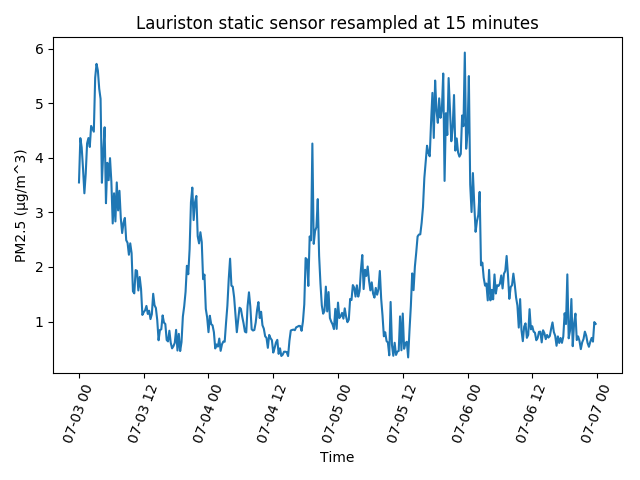
\includegraphics[width=\textwidth]{images/static_sensor_lauriston_resampled_15_min.png}
\caption{Values resampled to 15 minutes}
\label{fig:resample_15}
\end{subfigure}%
%
\hfill
%
\begin{subfigure}[t]{0.5\textwidth}
\centering
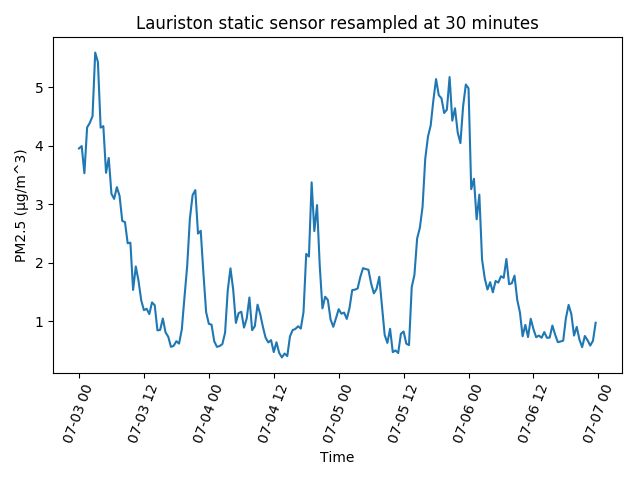
\includegraphics[width=\textwidth]{images/static_sensor_lauriston_resampled_30_min.png}
\caption{Values resampled to 30 minutes}
\label{fig:resample_30}
\end{subfigure}

\bigskip 

\begin{subfigure}[t]{0.5\textwidth}
\centering
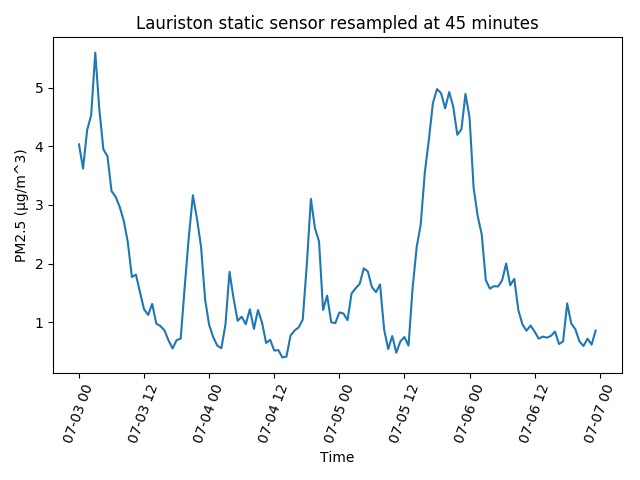
\includegraphics[width=\textwidth]{images/static_sensor_lauriston_resampled_45_min.png}
\caption{Values resampled to 45 minutes}
\label{fig:resample_45}
\end{subfigure}%
%
\hfill
%
\begin{subfigure}[t]{0.5\textwidth}
\centering
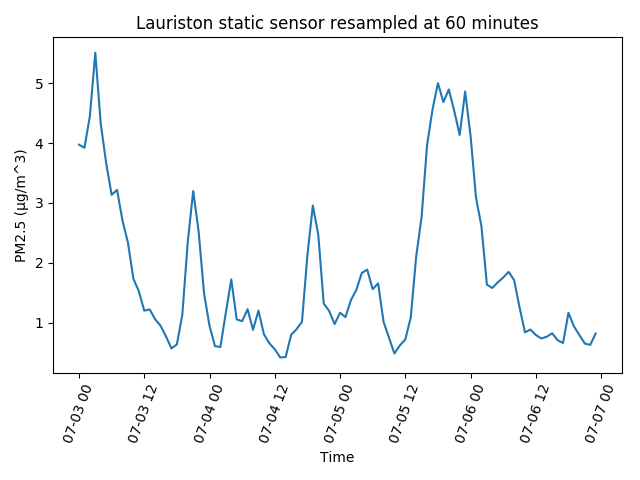
\includegraphics[width=\textwidth]{images/static_sensor_lauriston_resampled_60_min.png}
\caption{Values resampled to 60 minutes}
\label{fig:resample_60}
\end{subfigure}

\caption{Lauriston static sensor readings on dataset A}
\label{fig:resamples}
\end{figure*}


\begin{table}[h]
\centering
\resizebox{\textwidth}{!}{%
\begin{tabular}{c|c|c}
\textbf{Training method (MAE/MSE)} & \textbf{Predicting 15 minutes ahead} & \textbf{Predicting 60 minutes ahead} \\ \hline
Using 15 minute intervals & \textbf{0.159 / 0.076} & 0.254 / 0.156 \\ \hline
\begin{tabular}[c]{@{}c@{}}Using a 60-minute rolling mean every 15 minutes \\ (45 minutes overlap)\end{tabular} & 0.180 / 0.078 & 0.291 / 0.182
\end{tabular}%
}
\caption{MAE and MSE comparison of time windows and prediction distance}
\label{tab:distance_pred}
\end{table}

Results show that regardless of the prediction distance, 15 minutes ahead or 60 minutes ahead, using the 15 minute time window performs better than using a 60-minute rolling mean. It is also possible to observe that predicting 15 minutes into the future produces less error than 60 minutes ahead, as would be expected.

Figure \ref{fig:errorahead} illustrates the comparison of errors when only predictions are made (blue line) and when predicting and training is occurring (orange line). The blue line corresponds to the online model proposed because, at every step in the horizontal axis, the model is partially trained with the data seen in the window before. In contrast, the orange line shows the error increasing over time as the model was only trained at time window zero and the model tries to predict further into the future without the knowledge of the most recent data. In this Figure, we can observe the advantages of the online model to make shorter-term predictions, as the capability to adapt to very recent data by partially training more frequently allows the error to remain low over time.

\begin{figure}[h]
    \centering
    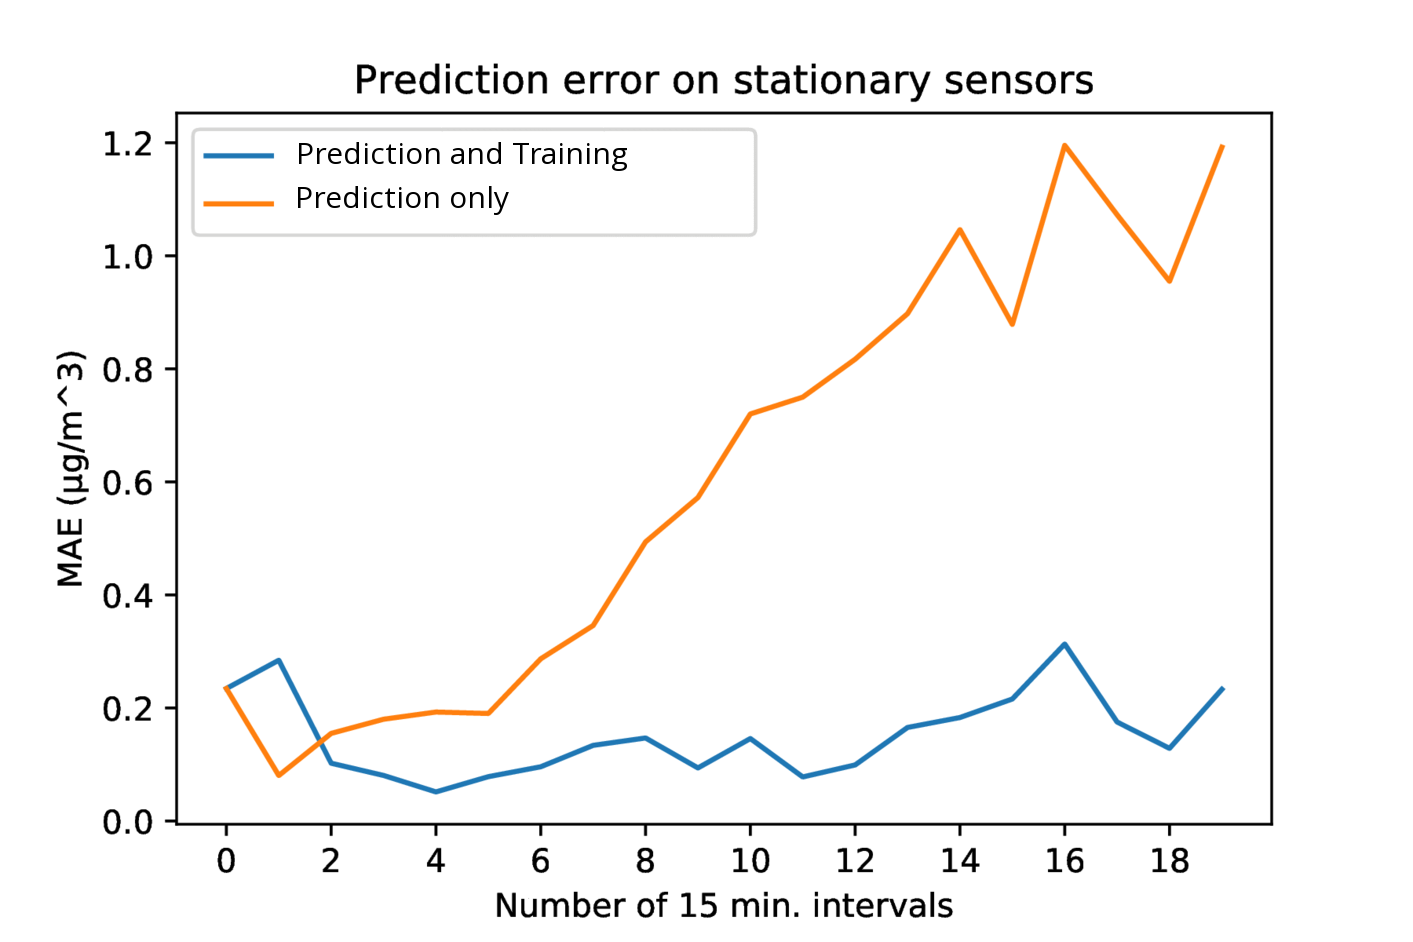
\includegraphics[width=0.8\textwidth]{images/prediction_error.png}
    \caption{Comparison between only predicting and predicting \& training (online) over time}
    \label{fig:errorahead}
\end{figure}

\section{Spatio-temporal Results and Analysis}
\label{chap:st_results}

The performance of the online spatio-temporal model is presented in this section. One of the novel parts of the model, the integration of mobile data in the online training phase of the model was compared to the model without mobile data included in the training. Tests were made by comparing the predictions with the values read in the corresponding time window and cell grid. Both datasets, A and B, were tested. Overfitting to the training set does not apply in this case as the ground truth of a prediction is data that the model has not yet seen given it is a time in the future (future of where the model is simulated to be). Results were summarised in Table \ref{tab:spatiotemporal}. The analysis of these results shows that including mobile data in training the model improves predictions by $14\%$ in dataset A and $20\%$ in dataset B. 
This improvement in performance can also be attributed to the fact that the data that is being tested is geographically close to observations that were known shortly before and the online model was able to adapt to them, making use of locality to improve predictions. As an example, imagine a person walking a path throughout the grid with a mobile sensor reading PM2.5 values. The values that person collected 15 minutes before the present will be spatially close to where the person is located in the present, and because the model was able to adapt quickly to the data collected 15 minutes ago, the predictions to that person are improved in the present.
It is also important to refer from Table \ref{tab:spatiotemporal} that the results are 19\% better than the baseline in dataset A defined in section \ref{chap:baselines} as 2.81.

Note that the model supports data of mobile sensors regardless of the way they were collected, such as walking, cycling, skating, and more. The locality advantage still applies in these cases because from the model's perspective the only change that occurs is the number of cell grids travelled in each time window, and consecutive time windows share nearby observed grid cells. In the datasets used, both walking and cycling data were available and used.

It is also possible to analyse these results from another perspective. Given that the MAE of the temporal model achieved on cells with static sensors in place is $0.159$ (from \ref{tab:distance_pred}), and the MAE of the spatio-temporal model on cells where mobile data was collected is $2.28$ (from \ref{tab:spatiotemporal}), we could extract two insights about the data: Firstly, would it be the case where the whole grid is filled with static sensors or data for all grid cells is available through static and mobile sensors, we could see the spatio-temporal MAE get closer to the temporal MAE. Secondly, we can identify the spatial interpolation as a significant source of error. Further experiments described in section \ref{improvement} try to improve that performance with success.



\begin{table}[H]
\centering
\resizebox{\textwidth}{!}{%
\begin{tabular}{c|c|l|c|l|}
\textbf{Training method} & \multicolumn{2}{c|}{\textbf{Dataset A}} & \multicolumn{2}{c|}{\textbf{Dataset B}} \\ \cline{2-5} 
\multicolumn{1}{l|}{} & \multicolumn{1}{l|}{\textbf{With mobile data}} & Without mobile data & \multicolumn{1}{l|}{\textbf{With mobile data}} & Without mobile data \\ \hline
Number of squares tested & \multicolumn{2}{c|}{369} & \multicolumn{2}{c|}{301} \\ \hline
Mean Absolute Error & \textbf{2.28} & \multicolumn{1}{c|}{2.65} & \textbf{1.21} & \multicolumn{1}{c|}{1.51} \\ \hline
\end{tabular}%
}
\caption{Spatio-temporal MAE results and Analysis}
\label{tab:spatiotemporal}
\end{table}

\subsection{Error visualisation}
In order to reduce the error, a script was developed to visualise the errors of the model. The result is presented in Figure \ref{fig:error_st}. In this Figure, it was detected that errors were mostly positive, indicating the model was mostly underpredicting the PM2.5 levels. If the model was not underpredicting, the green line, representing the mean of the errors would be on or close to zero, the red line drawn in the graph. That is not the case and indicates an improvement in accuracy could be achievable.


\begin{figure}[H] 
\centering
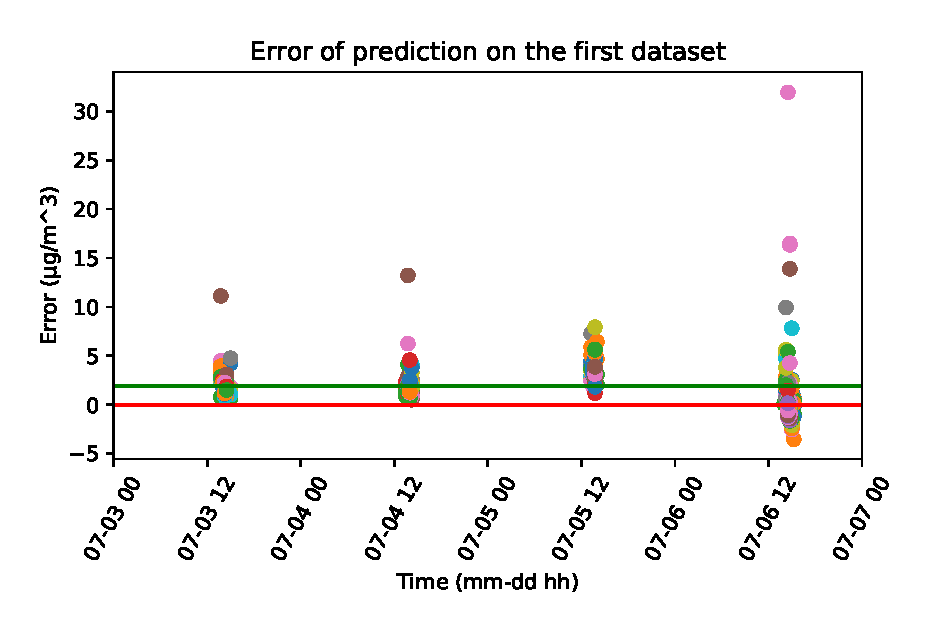
\includegraphics[width=\linewidth]{images/daily_error_with_line.eps} 
\caption{Errors of spatio-temporal model on dataset A. Different coloured dots represent the errors of the predictions made. The red line is defined as $Error = 0$ and the green line is defined by $Error = \textrm{\textit{Average of all errors displayed}} = 1.87 $.}
\label{fig:error_st}
\end{figure}

\section{Improvement using bias correction}
\label{improvement}

Using the known tendency for the model to underestimate predictions, an online correction system was produced to counter this imbalance. This aimed to further improve the performance of the prediction system without compromising the capability for the model to adapt in a real-time context.
The tests with the data correction algorithm were performed on dataset B, having dataset A just as training data to compute initial prediction errors. As seen in Figure \ref{fig:hist_mobile}, the mobile data available is sparse, and this method prevents a cold start of the algorithm. 
The correction algorithm's performance is compared to the base model performance without the algorithm in place. The aim is to achieve better performance than the base model, which, on dataset B produced MAE of 1.21.
Several experiments were implemented to analyse the improvement in performance on the base model. Three parameters were tested: The minimum amount of data stored to activate the error correction, the radius of the errors considered in the computation and the method of computing the amount of correction. 

Firstly, the minimum amount of data to prevent a cold start was tested, and results are presented in Table \ref{tab:min_threshold}. It is observable that the results remain relatively constant as the threshold increases and after that, when the threshold is big enough not to activate very often, the MAE gets closer to the MAE value without correction applied. Effectively, if a big enough threshold was chosen, the error correction would never activate and error output would be the same as the model without correction. There were no significant differences in setting the minimum amount of data needed to correct the prediction, therefore, a minimum of 3 errors was therefore chosen.

\begin{table}[]
\centering
\resizebox{\textwidth}{!}{%
\begin{tabular}{l|c|l|l|l}
 & \multicolumn{4}{c|}{Experiment performed with method "mean" and local data only} \\ \hline
 & \multicolumn{1}{l|}{\textbf{Minimum threshold = 3}} & Minimum threshold = 5 & Minimum threshold = 7 & \multicolumn{1}{l|}{Minimum threshold = 10} \\ \hline
\multicolumn{1}{c|}{Mean Absolute Error} & \textbf{1.293} & \multicolumn{1}{c|}{1.294} & \multicolumn{1}{c|}{1.294} & \multicolumn{1}{c|}{1.241} \\ \hline
\end{tabular}%
}
\caption{Minimum activation threshold experiment results}
\label{tab:min_threshold}
\end{table}

Secondly, three radii of data used for correction were tested. One where only data from the same cell would be used, referred to as using local data, one where adjacent cells would also be used, referred to as using neighbouring data and one where data from all cells would be used, referred to using global data. These three alternatives are represented in Figure \ref{fig:error_corrcections}.

\begin{figure}[h]
\centering
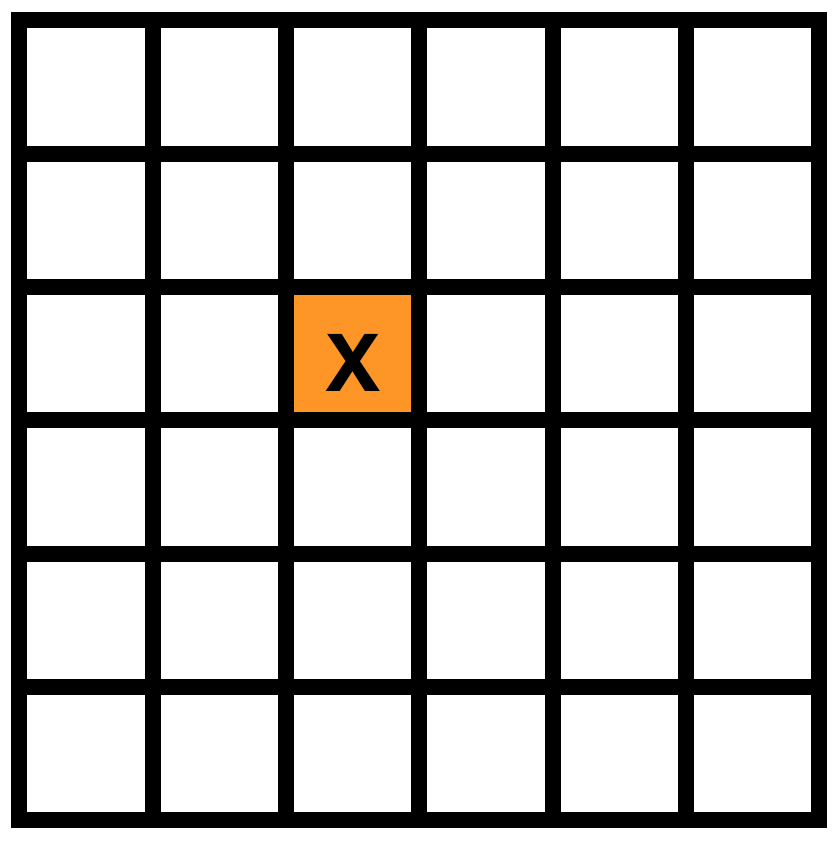
\includegraphics[width=.3\textwidth]{images/local_error.png}\hfill
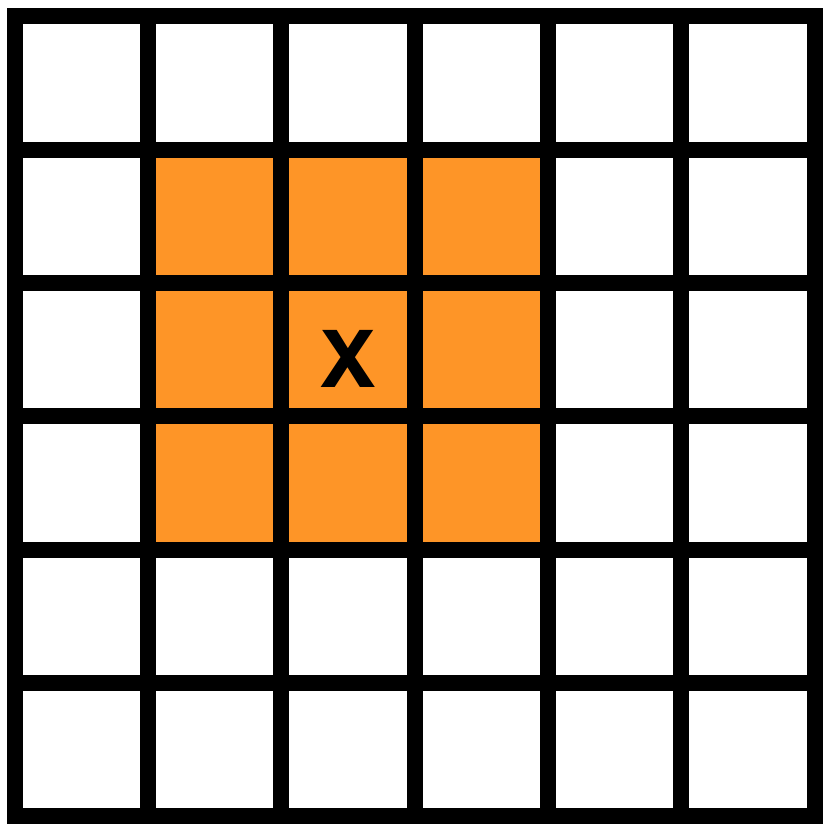
\includegraphics[width=.3\textwidth]{images/neighobour_error.png}\hfill
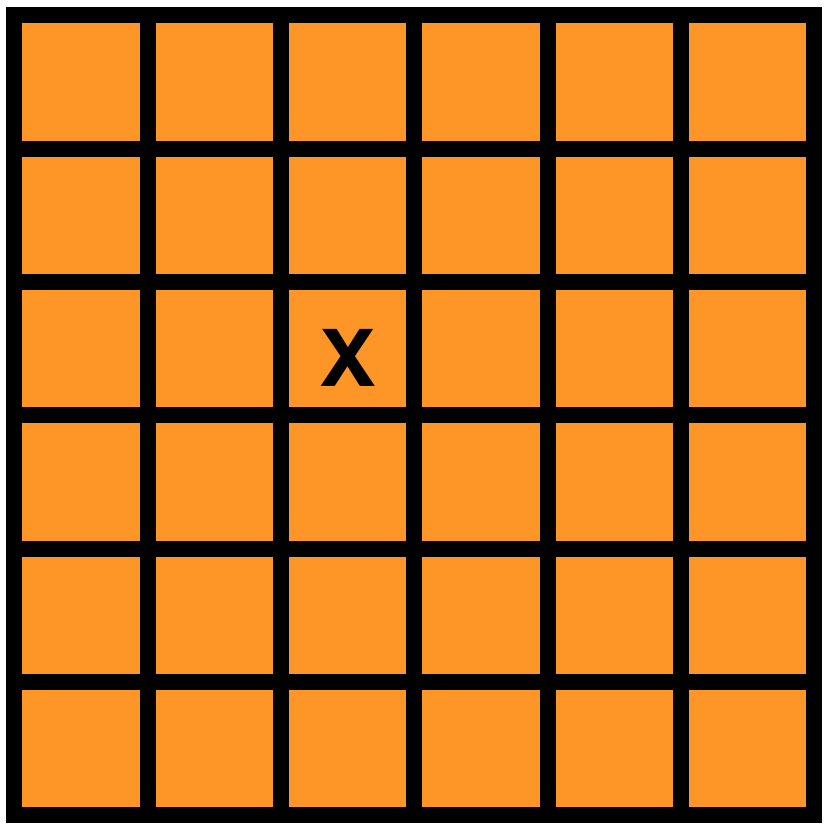
\includegraphics[width=.3\textwidth]{images/global_error.png}
\caption{Representation of errors used in local (left), neighboring (center) and global (right) scenarios, where "X" represents the location of the error correction that is being applied and orange filling represents the errors used to compute the error correction value.}
\label{fig:error_corrcections}

\end{figure}

\begin{table}[h]
\centering
\resizebox{\textwidth}{!}{%
\begin{tabular}{c|c|c|c|}
 & \multicolumn{3}{c|}{\begin{tabular}[c]{@{}c@{}}Experiment performed with minimum threshold = 3 \\ and mean as computation method\end{tabular}} \\ \hline
 & Local data & Neighboring data & \textbf{Global data} \\ \hline
Mean Absolute Error & 1.293 & 1.201 & \textbf{1.060} \\ \hline
\end{tabular}%
}
\caption{Results using different amounts of data for error correction}
\label{tab:mean_results}
\end{table}


The results of this experiment (Table \ref{tab:mean_results}) revealed that the error correction improvement is a very useful tool to make better predictions, but the tests show that there was not enough data on a small set of grid cells that allow the radius to be smaller than the entire grid. The more data is available in each cell, which is collected over time, the smaller the range can be and it would be interesting to investigate in the future whether this reduction of radius could even improve the predictions further, as each cell grid could have more detailed data about its specific behaviour in terms of errors.



Lastly, several methods of computing the amount of correction were tested: statistical properties such as mean and median, most recent error selection, and regression models such as linear regression and passive-aggressive regressor. Inspection of Table \ref{tab:local_global} shows that the machine learning models don't have enough data to be able to compare with statistical models, however, the Linear Regression model on global data was able to perform better than the model without correction even with the small amount of data. This indicates that, in the future, regression models could, with a more substantial amount of data data available, also improve the predictions, possibly even surpassing statistical models. Both the mean and the median methods were able to improve the performance of the predictions using global data, especially the median, which was the best performing correction method tested. This behaviour is likely to be due to the existence of outliers in dataset B, which the mean is more sensitive to than the median, making the median a more robust method to compute the correction to be applied. The error correction part of the model, therefore, improves performance by 22\% compared to the same model without error correction.

\begin{table}[h]
\centering
\resizebox{\textwidth}{!}{%
\begin{tabular}{c|c|c|}
 & \multicolumn{2}{c|}{Experiment performed with minimum threshold = 3} \\ \hline
Mean Abolute Error (MAE) & \multicolumn{2}{c|}{Data used} \\ \hline
Method of correction calculation & Local data & \textbf{Global data} \\ \hline
Last value seen & 1.452 & - \\
Mean & 1.293 & \textbf{1.060} \\
\textbf{Median} & 1.226 & \textbf{0.948} \\
Passive-Aggressive Regression & 6.212 & 3.700 \\
Linear Regression & 5.352 & \textbf{1.116}
\end{tabular}%
}
\caption{Comparison of different correction calculation methods. The results highlighted correspond to those that improve the model.}
\label{tab:local_global}
\end{table}


